\documentclass[seminar,english,m,frames]{AIGpaper}
% Please read the README.md file for additional information on the parameters and overall usage of AIGpaper

%%%% Package Imports %%%%%%%%%%%%%%%%%%%%%%%%%%%%%%%%%%%%%%%%%%%%%%%%%%%%%%%%%%%%%%%%%
\usepackage{graphicx}					    % enhanced support for graphics
\usepackage{tabularx}				      	% more flexible tabular
\usepackage{amsfonts}					    % math fonts
\usepackage{amssymb}					    % math symbols
\usepackage{amsmath}					    % overall enhancements to math environment

%%%% optional packages
\usepackage{tikz}                           % creating graphs and other structures
\usetikzlibrary{arrows,positioning, shapes.geometric}
\tikzset{
    %Define standard arrow tip
    >=stealth',
    %Define style for argument
    args/.style={circle, minimum size=0.9cm,draw=black, thick,fill=white},
}


%%%% Author and Title Information %%%%%%%%%%%%%%%%%%%%%%%%%%%%%%%%%%%%%%%%%%%%%%%%%%%
\author{Alexander Köhn}
%TODO Correct title of paper
\title{Basic Possibilistic Logic: Examples and Visualization}

%%%% Abstract %%%%%%%%%%%%%%%%%%%%%%%%%%%%%%%%%%%%%%%%%%%%%%%%%%%%%%%%%%%%%%%%%%%%%%


%TODO Ask if German Abstract is necessary
%\germanabstract{}

%TODO Write Abstract
% use this if the document is written in english
\englishabstract{
Lorem ipsum dolor sit amet, consetetur sadipscing elitr, sed diam nonumy eirmod tempor invidunt ut labore et dolore magna aliquyam erat, sed diam voluptua. At vero eos et accusam et justo duo dolores et ea rebum. Stet clita kasd gubergren, no sea takimata sanctus est Lorem ipsum dolor sit amet. Lorem ipsum dolor sit amet, consetetur sadipscing elitr, sed diam nonumy eirmod tempor invidunt ut labore et dolore magna aliquyam erat, sed diam voluptua.
}


\begin{document}

\maketitle % prints title and author information, as well as the abstract 


% Email Korrespondenz
% Eine Ausarbeitung der Beispiele aus dem Originalpapier würde ich für Ihre Ausarbeitung sehr begrüßen. Auch die Erarbeitung neuer Beispiel klingt sehr gut. Grundsätzlich sollte Ihre Ausarbeitung wenigstens die formale Präsentation von Syntax und Semantik possibilistischer Logik, sowie dazu notwendige Motivation und Beispiele enthalten. Darüberhinaus können Sie noch weitere Erweiterungen hinzufügen, sollten aber einen klaren Fokus setzen und nicht zu sehr in die Breite gehen.
% ===================== Beginning of the actual text section =====================

% Structure
% paper should not exceed 12 pages
% Introduce and explain the logic
% Relation to artificial intelligence
% Syntax and semantics
% Examples and porperties
%
\section{Introduction}
% This part motivates your whole document. You describe your goal and research questions on a (semi-)informal level. To do so, you have to present to the reader information on the research area and how your goals and questions are connected to the state of the art. You explain what you will do in your paper and how; furthermore, you explain why your work is relevant. At the end of your introduction, you describe how your document is organized textually. Keep the language in this part such that a non-expert in the field can (roughly) understand the goals and approaches of your text.
The goal of this paper is to introduce Basic Possibilistic Logic with examples and visualization. The focus of this paper is on introducing common and new examples with more explanation and visualization. In this paper we will only focus on Basic Possibilistic Logic. \\
This work is structured as follows. In Section \ref{Fundamentals} Basic Possibilistic Logic is explained with its Preliminaries for understanding the syntax and semantics of the logic. Before the core part of this paper the section \ref{DifferencesClassical} compares Possibilistic Logic with classical Logic and the section \ref{RelationAI} relates Possibilistic Logic with Artificial Intelligence. The Section \ref{Examples} shows the use of Basic Possibilistic Logic with multiple examples and graphical explanations. The last Section \ref{Conclusion} discusses the results of the previous sections.


%Possibilistic logic is a weighted logic that handles uncertainty in a qualitative way by adding certainty to classical logic formulas. Its strength lies in modeling uncertainty and its ability to deal with inconsistency.

%\subsection{Motivation}
%\subsection{Objectives of the paper}
%\subsection{Structure of the paper}

%\section{Preliminaries}
% The preliminaries introduce the research context of your document and the general prior work you make use of. You describe the theories and methodologies on which your work is built upon. Also, priorly existing algorithms and results you will make use of later will be presented here. Ensure that the preliminaries focus on the relevant aspects and keep an appropriate weight in the presentation. While it is often advisable to repeat basic results if they are only of marginal importance for your contributions, they should be presented only briefly. In contrast, when your contributions heavily use results from the literature, you should explain these results in detail.

\section{Fundamentals of Basic Possibilistic Logic} \label{Fundamentals}
As a main source for this introduction section the overview chapter: Possibilistic Logic - An Overview from the authors Dubois and Prade \cite{dubois2014possibilistic} is used. This section gives a short overview of Basic Possibilistic Logic. For more information, the work \cite{dubois2014possibilistic} is referred. \\
In this section we will first introduce main concepts of Possibility Theory. These concepts are necessary to understand Possibilistic Logic. Going further Basic Possibilistic Logic is introduced with the syntac, axioms, inference rules and semantic aspects.
\subsection{Introduction to Possibility Theory}
In the following basic concepts of Possibility theory are introduced which were first ligned out in \cite{zadeh1978}. Possibility theory is explained in detail in \cite{dubois2023possibility}. First the possibility distribution is introduced and second the basic set functions of Possibility theory which model the Possibility and necessity of events.
\subsubsection{Possibility Distribution}
A possibility distribution is a function \( \pi \) that maps elements from a set of states \( U \) to a totally ordered scale \( S \), where the highest value is 1 and the lowest is 0, see \cite{dubois2014possibilistic}:
\[
\pi: U \to S.
\]
The value \( \pi(u) \) indicates the degree of possibility assigned to the state \( u \). This function represents the agent's knowledge and helps differentiate between states that are more or less plausible. A state \( u \) is impossible if \( \pi(u) = 0 \), whereas it is considered fully possible if \( \pi(u) = 1 \). \\
%A distribution $ \pi $ is at least as specific as $ \pi' $ if
%\[
%\pi(u) \leq \pi'(u), \quad \forall u \in U.
%\]
%An agent has complete knowledge if the possibility of one state is 1 and the possibility of all other states is 0. Complete ignorance is given it the possibility of all states is 1.
%The Principle of minimal specificity states that any hypothesis not known to be impossible cannot be ruled out. It is a minimal commitment, cautious, information principle.
\subsubsection{Possibility and Necessity Functions}
If we want to know if the event $ A $ occurs we can respond in possibility theory with two measures calculated from the possibility distribution to $ A $.  $ A $ is a subset of states. The two measures are the possibility and the necessity of an event, see \cite{dubois2014possibilistic}. \\ 
The Possibility is defined as $ \Pi(A) = \sup_{u \in A} \pi \left( u \right) $. It is the maximum of possibility of all the states of $ A $. The Possibility evaluates the extent to which $ A $ is consistent with $ \pi $. Possibility measures satisfy the characteristic maxitivity property $ \Pi \left( A \cup B \right)  = \max \left( \Pi \left( A \right), \Pi \left(  B \right) \right) $. \\
The Necessity is defined as $ N(A) = \inf_{u \notin A} \left( 1 - \pi \left( u \right) \right) $. It is the minimum of the inversed possibility value of all states which are not in $ A $. The Necessity evaluates the extent to which $ A $ is certainly implied by $ \pi $. Necessity measures satisfy the characteristic minimization property $ N \left( A \cap B \right)  = \min \left( N \left( A \right) , N \left( B \right) \right) $. The minimization property expresses that to be certain about $ A $ and $ B $, one has to be certain about $ A $ and to be certain about $ B $. \\
The duality of the two measures is expressed as $ N \left( A \right)  = 1 - \Pi \left( A^c \right) $, where $ A^c $ is the complement of $ A $.

% Note also that we only have N(A?B) ? max(N(A),N(B)).This goes well with the idea that one may be certain about the event A?B, without being really certain about more specific events such as A and B.
\subsection{Formal foundations of Basic Possibilistic Logic}
In the following the foundations of Basic Possibilistic Logic are layed out. First the syntax is introduced. Second the axioms of this logic are derived and third the inference rules are explained. The last part covers the semantic aspects of the Logic.
\subsubsection{Syntax}
A basic possibilistic logic formula is represented as:
\[
(a, \alpha)
\]
where \(a\) is a classical logic formula (e.g., \(p \to q\)) and \(\alpha \) is the certainty level (minimum necessity degree of \( a \)). It can be viewed as a lower bound of a necessity measure. The pair $ \left( a , \alpha \right) $ is understood as $ N \left( a \right) > \alpha $. 
We can interpret that the formula $ a $ is at least certain to degree $ \alpha $. The higher $ \alpha $, the stronger the belief in $ a $. For example \((b \to f, 0.9)\) means that birds fly with certainty $ 0.9 $.
\subsubsection{Axioms}
The axioms of Possibilistic Logic are those of propositional logic. In the following the inference rules of basic possibilistic logic will be explained. The Certainty weakening rule states that if a formula is valid with a high certainty level, it is also valid with any lower certainty level.  If a formula holds with a certainty level $ \alpha $, it automatically implies that it holds with any lower level of certainty $ \beta $ because we are being less demanding, see equation  \ref{Eq:Certainty_weakening}.
\begin{equation} \label{Eq:Certainty_weakening}
	\text{If } \beta \leq \alpha, \quad (a, \alpha) \vdash (a, \beta)
\end{equation}
The Modus ponens rules states that if $ a $ to $ b $ is true with certainty level $ \alpha $, and $ a $ is also true with certainty level $ \alpha $ then $ b $ must be true with certainty level $ \alpha $, see equation  \ref{Eq:Modus_ponens}.
\begin{equation}\label{Eq:Modus_ponens}
	(\neg a \lor b, \alpha), (a, \alpha) \vdash (b, \alpha), \quad \forall \alpha \in (0, 1]
\end{equation}
In classical logic, the resolution rule allows us to combine two clauses that share a literal to eliminate that literal and infer a new clause. In possibilistic logic, the resolution rule preserves the certainty level $ \alpha $, because the inferred formula $ b \lor c $ cannot be more certain than the least certain premise, see equation \ref{Eq:Resolution}.
\begin{equation}\label{Eq:Resolution}
	(\neg a \lor b, \alpha), \quad (a \lor c, \alpha) \vdash (b \lor c, \alpha)
\end{equation}
The weakest link resolution rule extends the resolution rule by  the concept of different certainty levels $ \alpha $ and $ \beta $ in the premises. The weakest link resolution reflects the idea that the certainty of the conclusion cannot exceed the weakest certainty of the premises. If one of the premises is less certain, it becomes the bottleneck for the certainty of the conclusion, see equation \ref{Eq:Weakest_link_resolution}.
\begin{equation}\label{Eq:Weakest_link_resolution}
	(\neg a \lor b, \alpha), \quad (a \lor c, \beta) \vdash (b \lor c, \min(\alpha, \beta))
\end{equation}
\subsubsection{Inference Rules}
We can define a possibilistic knowledge base as a collection of possibilistic formulas, see equation \ref{Eq:Knowledge_base}. 
\begin{equation}\label{Eq:Knowledge_base}
	\Gamma = \{(a_i, \alpha_i), i = 1, \dots, m\}
\end{equation}
Further we can define the $ \alpha $-cut of knowledge base, see equation \ref{Eq:Knowledge_base_cut}. It only contains those formulas from the origin knowledge base with a certainty level of at least $ \alpha $. It has a nested structure where the $ \alpha $ knwoledge base is a part of the $ \beta $ knowledge base if $ \alpha $ is higher than $ \beta $.
\begin{equation}\label{Eq:Knowledge_base_cut}
	\Gamma_\alpha = \{(a_i, \alpha_i) \in \Gamma \mid \alpha_i \geq \alpha\}
\end{equation}
A possibilistic inference \((a, \alpha)\) depends only on formulas with certainty levels \(\geq \alpha\), see equation \ref{Eq:Inference}.
\begin{equation}\label{Eq:Inference}
	\Gamma \vdash (a, \alpha) \iff \Gamma_\alpha \vdash (a, \alpha)
\end{equation}
If we want to infer from the knowledge, we can only look on the formulas with a certainty of at least $ \alpha $. This means that a inference is only valid if it is valid with the $ \alpha $-cut of a knowledge base. \\
An important attribute of knowledge bases is the inconsistency level. It is the highest certainty level at which the knowledge base becomes inconsistent. The properties of the inconsistency level show that all formulas which have a higher certainty level than the inconsistency level are safe form inconsistency, see equation \ref{Eq:Inconsistency_level}.
\begin{equation}\label{Eq:Inconsistency_level}
	\text{inc-l}(\Gamma) = \max\{\alpha \mid \Gamma \vdash (\bot, \alpha)\}
\end{equation}
\subsubsection{Semantic Aspects}
The semantics of possibilistic logic, as introduced in \cite{Dubois1994}, is based on the concepts of possibility distributions, weak possibility measures, and strong necessity measures. \\
Consider a possibilistic logic formula \((a, \alpha)\), representing the constraint \(N(a) \geq \alpha\). The semantics of this formula is expressed using a possibility distribution \(\pi(a, \alpha)\), defined as:
\[
\pi(a, \alpha)(\omega) = 
\begin{cases} 
	1 & \text{if } \omega \models a, \\
	1 - \alpha & \text{if } \omega \models \neg a.
\end{cases}
\]
The intuitive interpretation is that models of \(a\) are fully possible (\(\pi = 1\)), while counter-models of \(a\) are less possible as \(\alpha\) increases. When \(\alpha = 0\), the formula \((a, 0)\) provides no additional information and can be ignored.\\
The associated necessity measure satisfies:
\[
N_{a, \alpha}(a) = \alpha,
\]
and \(\pi(a, \alpha)\) is the least informative possibility distribution that satisfies this constraint.
\section{Differences from classical logic} \label{DifferencesClassical}
Possibilistic logic extends classical logic to address reasoning under uncertainty, offering mechanisms to represent degrees of belief and certainty. This section highlights the fundamental differences between the two logical frameworks, focusing on their semantics, expressive power, and handling of inconsistency.

\subsection{Representation of Uncertainty}

Classical logic operates within a binary truth-value system where every statement is either true (\(1\)) or false (\(0\)) \cite{Boole1854}. This simplicity facilitates precise reasoning but limits the capacity to model uncertainty or graded beliefs. For instance, in classical logic, if \(p\) is true, the disjunction \(p \lor q\) is true regardless of \(q\).

In contrast, possibilistic logic incorporates a certainty degree \(\alpha \in [0, 1]\) into formulas. A formula \((a, \alpha)\) encodes the constraint \(N(a) \geq \alpha\), where \(N(a)\) is a necessity measure representing the certainty of \(a\). As Dubois et al. explain, this framework allows for "a more nuanced reasoning where uncertainty is explicitly quantified" \cite{Dubois1994}. This makes possibilistic logic particularly suitable for applications such as decision-making and expert systems.

\subsection{Semantics}

The semantics of classical logic are based on truth assignments, where a model is a complete assignment of truth values to all propositions. A formula is true if it holds in all models satisfying the formula \cite{Tarski1941}.

Possibilistic logic employs possibility distributions to rank interpretations by their plausibility. A possibility distribution \(\pi(\omega)\) assigns a degree of possibility \([0, 1]\) to each interpretation \(\omega\). Models of a formula \(a\) have maximum possibility (\(\pi = 1\)), while countermodels have reduced possibility proportional to the certainty level \(\alpha\). This richer semantic framework accommodates reasoning with uncertainty and vagueness \cite{Dubois1994}.

\subsection{Handling Inconsistency}

Classical logic adopts a strict approach to inconsistency: the presence of a contradiction (\(a \land \neg a\)) renders the entire knowledge base invalid, allowing any formula to be derived \cite{Priest2008}.

Possibilistic logic, on the other hand, quantifies inconsistency. The inconsistency degree of a knowledge base reflects the extent to which it is contradictory. As Dubois et al. note, possibilistic logic "enables reasoning to proceed by prioritizing more certain information and disregarding less certain, conflicting data" \cite{Dubois1996}. This feature makes it robust for reasoning in incomplete and inconsistent environments.

\subsection{Expressiveness}

Classical logic excels in deterministic reasoning, where propositions are crisp and well-defined. It forms the foundation of mathematics, formal verification, and theoretical computer science \cite{Russell1903}. However, it cannot represent graded uncertainty.

Possibilistic logic extends the expressive power of classical logic by introducing mechanisms to model partial beliefs and degrees of certainty. This capability is crucial in fields like artificial intelligence, where uncertainty is inherent to problem-solving \cite{Zadeh1978}.

\subsection{Entailment}

Entailment in classical logic is binary: \(\Delta \models a\) indicates that \(a\) is true in all models of \(\Delta\). For example, if \(\Delta = \{p, p \to q\}\), then \(q\) is entailed if \(p\) is true \cite{Tarski1941}.

In possibilistic logic, entailment is graded. \(\Delta \models (a, \alpha)\) implies that \(a\) is true in all interpretations with at least the certainty level \(\alpha\). This certainty-based entailment enables reasoning about the strength of conclusions, a key feature in real-world applications \cite{Dubois1994}.

\subsection{Applications}

Classical logic is well-suited for deterministic problems with clear, unambiguous rules, such as mathematical reasoning and logic programming \cite{Boole1854}. 

Possibilistic logic, by contrast, is tailored for reasoning under uncertainty. Its ability to handle graded beliefs makes it a powerful tool in domains like artificial intelligence, decision support systems, and fuzzy logic applications. For example, possibilistic logic integrates seamlessly with fuzzy systems to facilitate approximate reasoning \cite{Dubois1994, Zadeh1978}.

\subsection{Summary}

The primary distinctions between classical and possibilistic logic are summarized in Table~\ref{tab:logic_comparison}.

\begin{table}[h!]
	\centering
	\caption{Comparison of Classical Logic and Possibilistic Logic}
	\label{tab:logic_comparison}
	\begin{tabular}{|l|l|l|}
		\hline
		\textbf{Aspect}            & \textbf{Classical Logic}                  & \textbf{Possibilistic Logic}               \\ \hline
		Truth Values               & Binary (\(0, 1\))                        & Graded (\([0, 1]\))                        \\ \hline
		Semantics                  & Truth Assignments                        & Possibility Distributions                  \\ \hline
		Uncertainty Handling       & Not Supported                           & Explicitly Represented                     \\ \hline
		Inconsistency Handling     & All-or-Nothing                          & Quantified and Managed                     \\ \hline
		Applications               & Deterministic Problems                  & Uncertain or Vague Reasoning               \\ \hline
		Entailment                 & Binary                                  & Certainty-Based                            \\ \hline
	\end{tabular}
\end{table}

Possibilistic logic, by building upon classical logic, provides the means to address the limitations of classical reasoning in uncertain and inconsistent environments. As Dubois et al. summarize, "its ability to combine logical precision with graded uncertainty makes it a valuable tool for real-world reasoning tasks" \cite{Dubois1994}.

\section{Relation to Artificial Intelligence} \label{RelationAI}
Possibilistic logic has a significant role in the field of artificial intelligence (AI), where reasoning under uncertainty is a fundamental challenge. Unlike classical logic, which assumes a deterministic world, possibilistic logic provides a framework to model and reason about incomplete, inconsistent, or uncertain information. This capability makes it particularly relevant to AI systems that must operate in real-world environments.

\subsection{Reasoning Under Uncertainty}

In AI, systems frequently encounter scenarios where the available information is uncertain or imprecise. Classical logic, which relies on binary truth values, is insufficient for such cases. Possibilistic logic addresses this limitation by introducing graded measures of certainty and possibility. Each formula in possibilistic logic is associated with a certainty degree, allowing AI systems to represent and process partial beliefs \cite{Dubois1994}.

For example, in expert systems, possibilistic logic can encode the varying reliability of rules provided by human experts. A rule with a higher certainty degree is given more weight in inference processes, enabling the system to prioritize more reliable information \cite{Prade1985}.

\subsection{Handling Inconsistency}

Inconsistencies are inevitable in real-world AI applications, particularly when combining knowledge from multiple sources. Classical logic treats any inconsistency as catastrophic, rendering the entire knowledge base unusable. Possibilistic logic, by contrast, quantifies inconsistency and allows reasoning to continue by prioritizing more certain information \cite{Dubois1996}. This feature is crucial for applications such as multi-agent systems and knowledge integration, where conflicting data is common.

\subsection{Applications in AI}

Possibilistic logic has been applied in various AI domains, demonstrating its versatility and utility. Key applications include:

\begin{itemize}
	\item \textbf{Decision Support Systems:} Possibilistic logic enables decision-making under uncertainty by modeling degrees of belief and their impact on outcomes. This is particularly useful in medical diagnosis and risk assessment systems \cite{Benferhat1997}.
	\item \textbf{Natural Language Processing (NLP):} Uncertainty is inherent in NLP tasks, such as semantic analysis and information retrieval. Possibilistic logic provides a robust framework for modeling linguistic uncertainty and ambiguity \cite{Dubois1994}.
	\item \textbf{Fuzzy Systems:} Possibilistic logic integrates seamlessly with fuzzy logic to facilitate approximate reasoning, making it a natural choice for control systems and robotics \cite{Zadeh1978}.
\end{itemize}

\subsection{Relation to Other AI Frameworks}

Possibilistic logic is closely related to other uncertainty reasoning frameworks in AI, such as probabilistic reasoning and fuzzy logic. While probabilistic approaches focus on quantifying uncertainty in terms of likelihoods, possibilistic logic emphasizes qualitative reasoning based on plausibility and necessity measures \cite{Dubois1988}. This distinction makes possibilistic logic particularly suited to scenarios where precise probability distributions are unavailable or unnecessary.

Moreover, possibilistic logic complements fuzzy logic by providing a logical foundation for reasoning about fuzzy sets. As Zadeh \cite{Zadeh1978} observed, the integration of fuzzy logic and possibilistic reasoning enables more sophisticated modeling of real-world problems, particularly those involving vague or imprecise concepts.

\subsection{Conclusion}

The ability of possibilistic logic to handle uncertainty, inconsistency, and imprecision makes it a valuable tool in AI. By extending classical logic with measures of certainty and possibility, it bridges the gap between theoretical rigor and practical applicability in uncertain environments. As Dubois and Prade note, "possibilistic logic combines logical precision with the flexibility required for real-world reasoning" \cite{Dubois1994}.


\section{Analysis and Development of Examples} \label{Examples}
In the following examples of the application of Possibilistic Logic are explained. First the Penguin Problem is used for understanding the logic better. Second a new Problem is introduced.
\subsection{The Penguin Problem}

One of the classical examples in non-monotonic reasoning is the Penguin Example, which highlights the need for reasoning under exceptions and uncertainty. In classical logic, general rules like "birds fly" lead to contradictions when exceptions, such as "penguins do not fly," are introduced. Possibilistic logic provides a structured way to handle such exceptions by associating rules with certainty levels and defining a preference ordering over possible worlds. \\
If the goal is to know if something flies or not we can use the default rules to generate a possibilistic logic base and to assign the rules graded certainties. With them we can apply our knowledge about the object and find out if it flies.
\subsubsection{Default Rules and Constraints}
The knowledge base consists of three default rules that represent generic knowledge about birds and penguins:
\begin{align*}
	d_1 &: b \rightarrow f \quad (\text{"Birds fly"}), \\
	d_2 &: p \rightarrow \neg f \quad (\text{"Penguins do not fly"}), \\
	d_3 &: p \rightarrow b \quad (\text{"Penguins are birds"}).
\end{align*}
From these default rules, a set of \textit{comparative possibility constraints} can be constructed:
\begin{align*}
	C_1 &: b \land f >_\Pi b \land \neg f \quad \text{(birds fly)}, \\
	C_2 &: p \land \neg f >_\Pi p \land f \quad \text{(penguins do not fly)}, \\
	C_3 &: p \land b >_\Pi p \land \neg b \quad \text{(penguins are birds)}.
\end{align*}
These constraints establish an ordering over possible worlds, prioritizing those that align with more general and certain rules. As the default rules clearly state with each constraint which world is more plausible.
\subsubsection{Possible Worlds and Possibility Distribution}
The propositional language for this example involves three predicates: $b$ (bird), $p$ (penguin), and $f$ (flies). The set of possible worlds, $\Omega$, corresponds to all truth-value assignments:
\begin{align*}
	\Omega = \{ \omega_0, \omega_1, \omega_2, \omega_3, \omega_4, \omega_5, \omega_6, \omega_7 \},
\end{align*}
where each $\omega_i$ represents a distinct combination of $(b, f, p)$. Based on the constraints, these worlds are ranked to reflect which interpretations are more plausible.
\begin{table}[h]
	\centering
	\begin{tabular}{c|c|c|c|c|c|c}
		World & $b$ (Bird) & $f$ (Flies) & $p$ (Penguin) & $d_1$: $b \to f$ & $d_2$: $p \to \neg f$ & $d_3$: $p \to b$ \\
		$\omega_0$ & 0 & 0 & 0 &  &  &  \\
		$\omega_1$ & 0 & 0 & 1 &  & true & false \\
		$\omega_2$ & 0 & 1 & 0 &  &  &  \\
		$\omega_3$ & 0 & 1 & 1 &  & false & false \\
		$\omega_4$ & 1 & 0 & 0 & false &  &  \\
		$\omega_5$ & 1 & 0 & 1 & false & true & true \\
		$\omega_6$ & 1 & 1 & 0 & true &  &  \\
		$\omega_7$ & 1 & 1 & 1 & true & false & true \\
	\end{tabular}
	\caption{Truth values of bird (\(b\)), flies (\(f\)), and penguin (\(p\)) for each world \(\omega_i\), and whether each world satisfies or violates the default rules.}
	\label{tab:worlds_rules}
\end{table}

\begin{align*}
	C_1 &: \max(\pi(\omega_6), \pi(\omega_7)) > \max(\pi(\omega_4), \pi(\omega_5)), \\
	C_2 &: \max(\pi(\omega_5), \pi(\omega_1)) > \max(\pi(\omega_3), \pi(\omega_7)), \\
	C_3 &: \max(\pi(\omega_5), \pi(\omega_7)) > \max(\pi(\omega_1), \pi(\omega_3)).
\end{align*}

Applying the principle of minimal specificity, we derive the following \textit{possibility levels}:
\begin{align*}
	\pi(\omega_0) &= \pi(\omega_2) = \pi(\omega_6) = 1, \\
	\pi(\omega_4) &= \pi(\omega_5) = \frac{2}{3}, \\
	\pi(\omega_1) &= \pi(\omega_3) = \pi(\omega_7) = \frac{1}{3}.
\end{align*}
This ranking captures the idea that worlds in which birds fly are more plausible than those in which they do not, except when dealing with penguins.
% Hasse Diagram
\paragraph*{1. World Ordering Lattice (Hasse Diagram)}
\begin{center}
	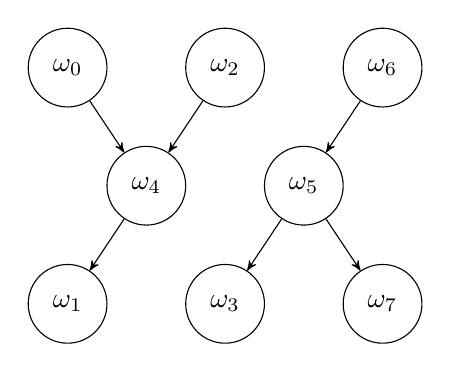
\begin{tikzpicture}[node distance=1.5cm, every node/.style={draw, circle, minimum size=1cm}]
		\node (w0) at (0,0) {$\omega_0$};
		\node (w2) at (2,0) {$\omega_2$};
		\node (w6) at (4,0) {$\omega_6$};
		
		\node (w4) at (1,-1.5) {$\omega_4$};
		\node (w5) at (3,-1.5) {$\omega_5$};
		
		\node (w1) at (0,-3) {$\omega_1$};
		\node (w3) at (2,-3) {$\omega_3$};
		\node (w7) at (4,-3) {$\omega_7$};
		
		% Draw edges
		\draw[->] (w0) -- (w4);
		\draw[->] (w2) -- (w4);
		\draw[->] (w6) -- (w5);
		
		\draw[->] (w4) -- (w1);
		\draw[->] (w5) -- (w3);
		\draw[->] (w5) -- (w7);
	\end{tikzpicture}
\end{center}

\paragraph*{Hasse Diagram with Justifications}

\begin{center}
	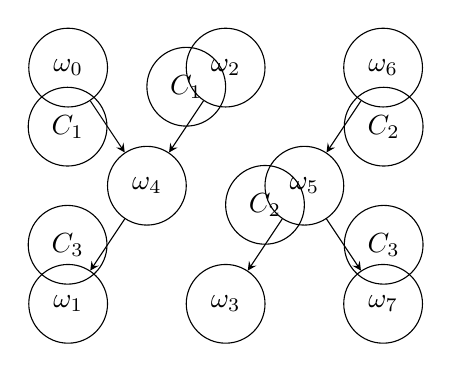
\begin{tikzpicture}[node distance=1.5cm, every node/.style={draw, circle, minimum size=1cm}, >=stealth]
		
		% Nodes
		\node (w0) at (0,0) {$\omega_0$};
		\node (w2) at (2,0) {$\omega_2$};
		\node (w6) at (4,0) {$\omega_6$};
		
		\node (w4) at (1,-1.5) {$\omega_4$};
		\node (w5) at (3,-1.5) {$\omega_5$};
		
		\node (w1) at (0,-3) {$\omega_1$};
		\node (w3) at (2,-3) {$\omega_3$};
		\node (w7) at (4,-3) {$\omega_7$};
		
		% Arrows with Labels
		\draw[->] (w0) -- (w4) node[midway, left] {$C_1$};
		\draw[->] (w2) -- (w4) node[midway, above] {$C_1$};
		\draw[->] (w6) -- (w5) node[midway, right] {$C_2$};
		
		\draw[->] (w4) -- (w1) node[midway, left] {$C_3$};
		\draw[->] (w5) -- (w3) node[midway, above] {$C_2$};
		\draw[->] (w5) -- (w7) node[midway, right] {$C_3$};
		
	\end{tikzpicture}
\end{center}

\subsubsection{Reasoning with Uncertain Information}

Possibilistic logic enables reasoning with uncertain and potentially conflicting information. Suppose we introduce the information that Tweety is a bird:
\begin{align*}
	F = \{ (b, 1) \} \quad \text{(Tweety is a bird with certainty 1)}.
\end{align*}
From the rule $(\neg b \lor f, 1/3)$ in the knowledge base $K$, we can infer:
\begin{align*}
	(\neg b \lor f, 1/3) \quad \text{and} \quad (b, 1) \vdash (f, \min(1, 1/3)) = (f, 1/3).
\end{align*}
Thus, we conclude that Tweety flies with a certainty level of $\frac{1}{3}$.

However, if new information states that Tweety is also a penguin:
\begin{align*}
	F = \{ (b,1), (p,1) \} \quad \text{(Tweety is a penguin with certainty 1)},
\end{align*}
then, using $(\neg p \lor \neg f, 2/3)$, we derive:
\begin{align*}
	(\neg p \lor \neg f, 2/3) \quad \text{and} \quad (p, 1) \vdash (\neg f, \min(1, 2/3)) = (\neg f, 2/3).
\end{align*}
Since we now have conflicting conclusions:
\begin{align*}
	(\neg f, 2/3) \quad \text{and} \quad (f, 1/3) \vdash (\bot, \min(2/3, 1/3)) = (\bot, 1/3),
\end{align*}
the system detects an inconsistency of level $\frac{1}{3}$. Given the principle that higher certainty information takes precedence, the inference that Tweety flies is suppressed, leading to the final conclusion:
\begin{align*}
	K \cup F \vdash (\neg f, 2/3),
\end{align*}
which means \textit{"Tweety does not fly"} with a certainty of $\frac{2}{3}$.



% Heatmap Bar Chart
\paragraph*{2. Possibility Levels of Worlds}
\begin{center}
	\begin{tikzpicture}
		\draw[->] (0,0) -- (8,0) node[right] {Worlds $\omega_i$};
		\draw[->] (0,0) -- (0,4) node[above] {Possibility $\pi(\omega_i)$};
		
		% Bars
		%\foreach \x/\h/\l in {0/3/$\omega_0, \omega_2, \omega_6$,
			%1.5/2/$\omega_4, \omega_5$,
			%3/1/$\omega_1, \omega_3, \omega_7$} {
			%\fill[blue!40] (\x,0) rectangle (\x+1, \h);
			%\node at (\x+0.5,\h+0.2) {\l};
		%}
	\end{tikzpicture}
\end{center}

% Flowchart for Reasoning
\paragraph*{3. Possibilistic Reasoning Flowchart}
\begin{center}
	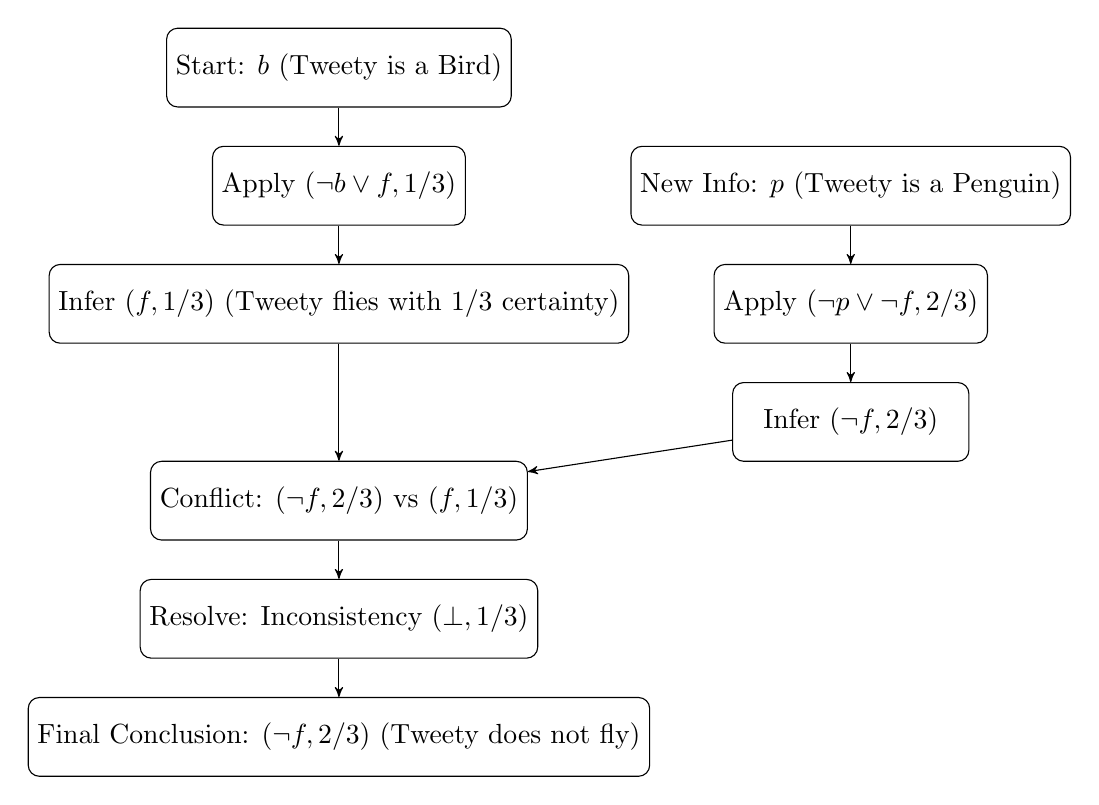
\begin{tikzpicture}[node distance=1.5cm, every node/.style={draw, rounded corners, minimum width=3cm, minimum height=1cm}]
		\node (start) {Start: $b$ (Tweety is a Bird)};
		\node (applyRule1) [below of=start] {Apply $(\neg b \lor f, 1/3)$};
		\node (inferF) [below of=applyRule1] {Infer $(f, 1/3)$ (Tweety flies with 1/3 certainty)};
		
		\node (newInfo) [right of=applyRule1, xshift=5cm] {New Info: $p$ (Tweety is a Penguin)};
		\node (applyRule2) [below of=newInfo] {Apply $(\neg p \lor \neg f, 2/3)$};
		\node (inferNotF) [below of=applyRule2] {Infer $(\neg f, 2/3)$};
		
		\node (conflict) [below of=inferF, yshift=-1cm] {Conflict: $(\neg f, 2/3)$ vs $(f, 1/3)$};
		\node (resolve) [below of=conflict] {Resolve: Inconsistency $(\bot, 1/3)$};
		\node (conclusion) [below of=resolve] {Final Conclusion: $(\neg f, 2/3)$ (Tweety does not fly)};
		
		% Arrows
		\draw[->] (start) -- (applyRule1);
		\draw[->] (applyRule1) -- (inferF);
		\draw[->] (newInfo) -- (applyRule2);
		\draw[->] (applyRule2) -- (inferNotF);
		\draw[->] (inferF) -- (conflict);
		\draw[->] (inferNotF) -- (conflict);
		\draw[->] (conflict) -- (resolve);
		\draw[->] (resolve) -- (conclusion);
	\end{tikzpicture}
\end{center}

\subsubsection{Implications for AI and Non-Monotonic Reasoning}

This example illustrates how possibilistic logic naturally handles non-monotonic reasoning by allowing more specific rules (e.g., "penguins do not fly") to override general ones ("birds fly"). Unlike classical logic, which would face contradictions, or probability theory, which requires precise distributions, possibilistic logic provides a qualitative approach to default reasoning. It enables AI systems to reason under uncertainty while maintaining a structured approach to resolving conflicts \cite{Dubois1994}.
\subsection{New Problem}


\section{Discussion and Conclusion} \label{Conclusion}
% In this part, you revisit the paper’s outline and summarise concisely the most important contributions of your document. It is advisable to connect your results with the research questions given in the introduction. Discuss relevant related work and potential future research questions and research problems that can be addressed in future work.
\subsection{Summary of findings}
\subsection{Limitations of the study}
\subsection{Outlook on future research}



\section{Example Figures and Tables}
Figure \ref{fig:af} shows an example of an abstract argumentation framework.

\begin{figure}[ht]
    \centering
    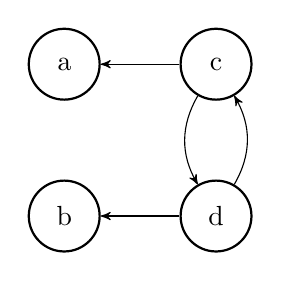
\begin{tikzpicture}[node distance=1cm]
    	\node[args](args1){a};
    	\node[args, below=of args1](args2){b};
    	\node[args, right=of args1](args3){c};
    	\node[args, right=of args2](args4){d};
    
        \path(args3) edge [->] (args1);
        \path(args3) edge [->, bend right] (args4);
        \path(args4) edge [->, bend right] (args3);
    	\path(args4) edge [->] (args2);
    \end{tikzpicture}
    \caption{An abstract argumentation framework.}
    \label{fig:af}
\end{figure}


\begin{table*}[ht]
\begin{center}
\begin{tabular}{lll}
\hline
1&2&3\\
4&5&6\\
\hline
\end{tabular}
\end{center}
\caption{Table caption.} \label{tab:t1}
\end{table*}



\subsection{Encoding Test}
Städte, Länder, Flüsse


% References
% In this part you list all literature your paper makes use of. Note that you should only include references that are actually referenced in the text. Take care that all references are complete (Authors, title, year of publication, publisher, etc.). Find further information on citing below.
\addreferences

\makestatement{1}

\end{document}
